\chapter{Implementation}\label{ch:implementation}
I dette afsnit vil der blive vist, hvordan løsningen er blevet implementeret. Koden er skrevet ud fra designklassediagrammet \ref{fig:designclassdiagram}, og benytter sig af de designmønstre som er vist i designklassediagrammet. Koden er skrevet i Java. 
De vigtigste metoder og designmønstre vil blive demonstreret, herunder parallelitet, singleton mønstret, database queries, og relevante algoritmer.

\todo{insert code snips, especially the stuff relevant to the database, our architecture, parallelity, and of course our regression algorithm.}


%algorithm stuff
En måde at beregne den optimale bestillingsmængde af en given vare, ud fra hvornår det betaler sig bedst, er ved at bruge en formel, bedre kendt som Economic Order Quantity (EOQ) Model \cite{EOQ}. Denne formel beregner bestillingsmængden ud fra efterspørgsel, pris per hjembestilling, kostpris per enhed og gennemsnitlig inventaromkostninger. Denne formel tager dog ikke højde for parametre såsom årstid, temperatur på dagen, antal solgt per dag, osv. For at kunne finde den optimale bestillingsmængde løbende, med et ønske om at altid have nok af alle varer på lager, kan parametre måned, temperatur, og daglige salg, bruges med regression. Regression er en teknik, hvorved man kan bestemme det statistiske forhold mellem to eller flere variabler, hvor ændringer i en dependent-variabel er associeret med, og afhænger af, én eller flere uafhængige variabler. Det bliver i dette projekt brugt til at forudsige f.eks. hvor mange Isbåde\cite{Isbåd} der skal bestilles over de næste uger, eller perioder. Når bestillingsmængden over tid når op til EOQ bestillingsmængden ville bestillingen af varen foretages.

%Shouldn't put in a figure of a formula we aren't using.
%\begin{landscape}
%    \begin{figure}[p]
%        \centering
%        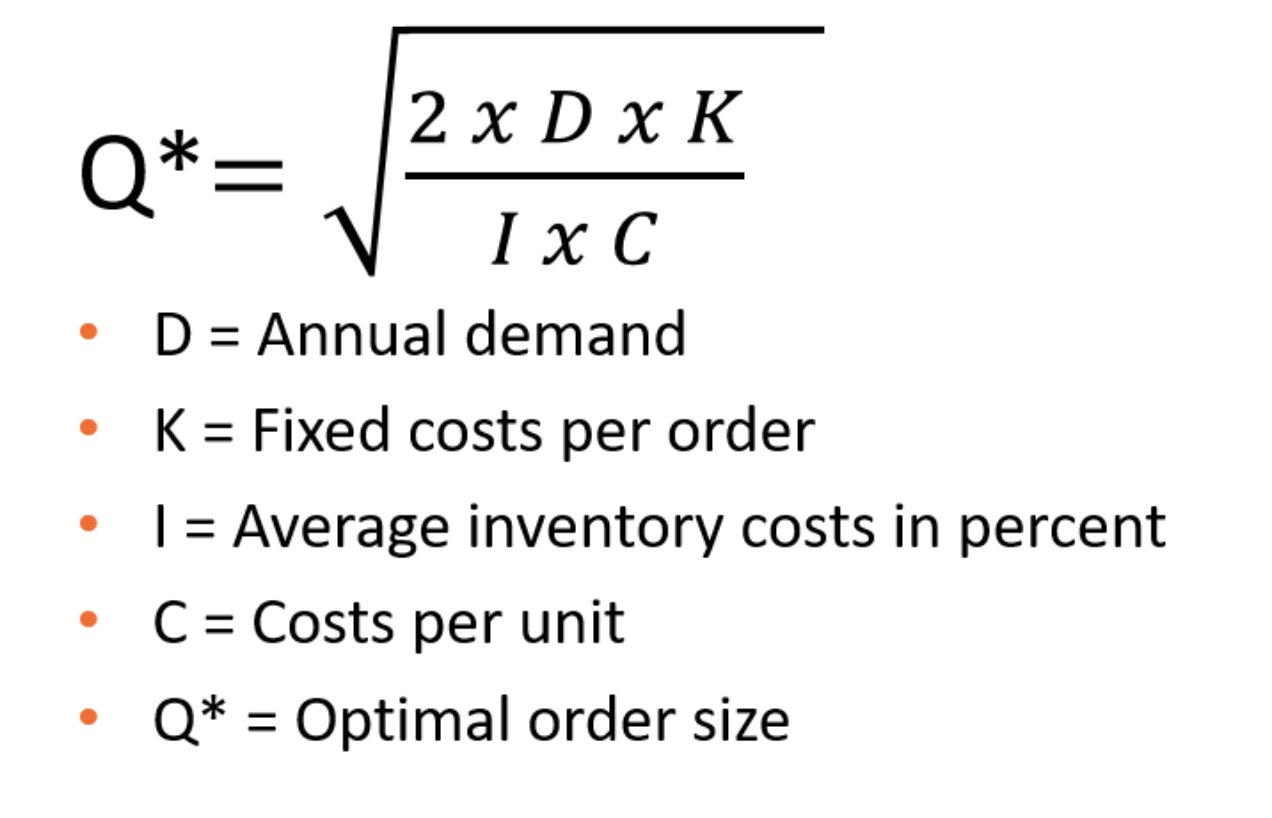
\includegraphics[width=\hsize]{figures/implementation/eoq.png}
%        \caption{EOQ formlen - Beregning af den optimale bestillingsmængde}
%        \label{fig:eoq}
%    \end{figure}
%\end{landscape}

I koden kan der så laves \verb|ProductLine| objekter, som lægges i \verb|PeriodicPlan| så der kan oprettes \verb|StorageOrder|s med de optimale bestillingsmængder. 
